\documentclass[12pt]{minimal}

\usepackage{graphicx}

\usepackage{tikz}

\usepackage[margin=0in, paperwidth=17.8cm, paperheight=5.3cm]{geometry}

\begin{document}

\centering
%\raisebox{4.5cm}{\sffamily{A}}
%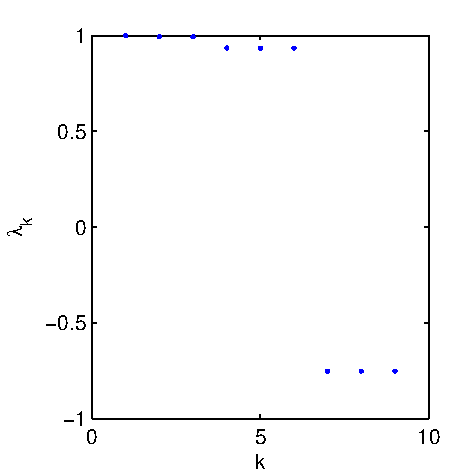
\includegraphics[width=5cm]{data1_evals}
\begin{tikzpicture}
	\node at (0,0) {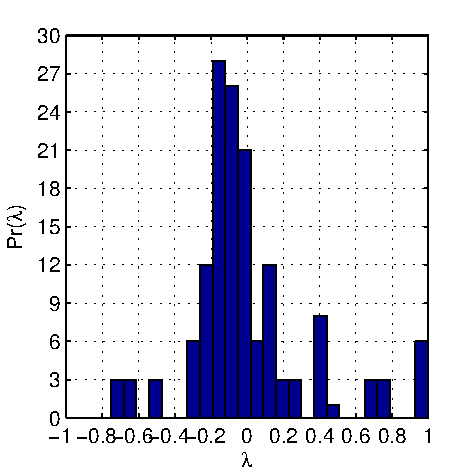
\includegraphics[width=5cm]{data1_evals_dist}};
	\node at (-2.5cm, 2cm) {\sffamily{A}};
%	\draw[<->, ultra thick, cyan] (-1.4cm, -1.9cm) -- (1.7cm, -1.9cm);
	\draw[<->, ultra thick, cyan] (-1.4cm, -1.85cm) -- (1.7cm, -1.85cm);
	\draw[->, ultra thick, red] (1.97cm, -0.5cm) -- (1.97cm, -1cm);
\end{tikzpicture}
%\raisebox{4.5cm}{\sffamily{B}}
%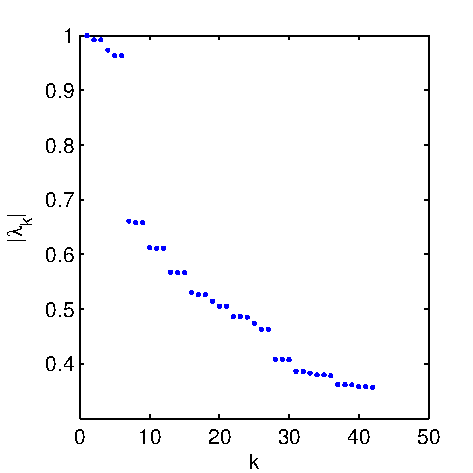
\includegraphics[width=5cm]{data2_evals}
\begin{tikzpicture}
	\node at (0,0) {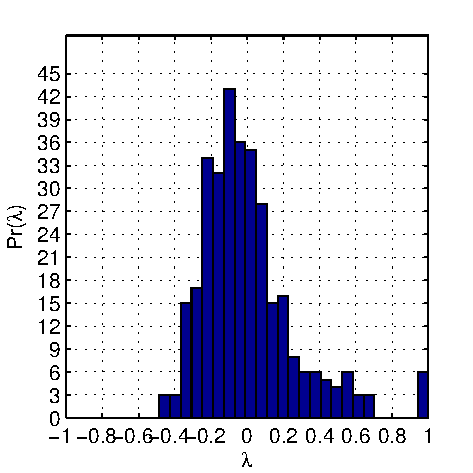
\includegraphics[width=5cm]{data2_evals_dist}};
	\node at (-2.5cm, 2cm) {\sffamily{B}};
	\draw[<->, ultra thick, cyan] (-1.2cm, -1.85cm) -- (1.5cm, -1.85cm);
	\draw[->, ultra thick, red] (1.97, -0.85cm) -- (1.97cm, -1.34cm);
\end{tikzpicture}
%\raisebox{4.5cm}{\sffamily{C}}
%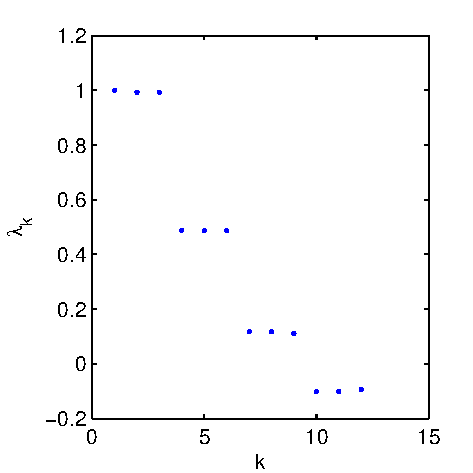
\includegraphics[width=5cm]{data3_evals}
\begin{tikzpicture}
	\node at (0,0) {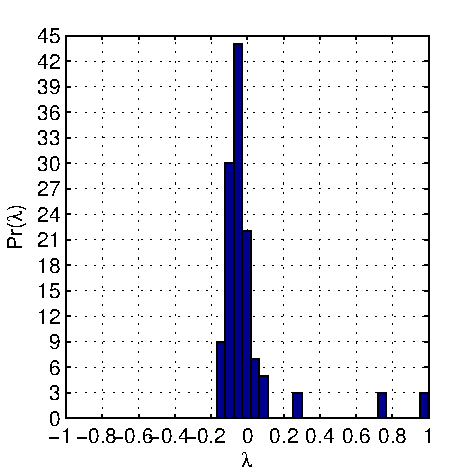
\includegraphics[width=5cm]{data3_evals_dist}};
	\node at (-2.5cm, 2cm) {\sffamily{C}};
	\draw[<->, ultra thick, cyan] (-0.25cm, -1.85cm) -- (0.35cm, -1.85cm);
	\draw[->, ultra thick, red] (1.97, -1.1cm) -- (1.97cm, -1.6cm);
	\draw[->, ultra thick, red] (1.52, -1.1cm) -- (1.52cm, -1.6cm);
	\draw[->, ultra thick, red] (0.64, -1.1cm) -- (0.64cm, -1.6cm);
\end{tikzpicture}

\end{document}